% ============================================================
%  Présentation du cours — Développement Web — Classe passerelle
%  PRÉSENTATION D'OUVERTURE (Beamer) — cfpt·i | Anne Terrier
%  À projeter au tout début de la première séance,
%  avant S01_presentation.tex (contenu technique de la semaine 1).
%  Charte graphique : cfpt·i (bleu accentBlue + jaune cfptYellow)
% ============================================================
\documentclass[aspectratio=169,11pt]{beamer}

\usepackage[T1]{fontenc}
\usepackage[utf8]{inputenc}
\usepackage[scaled=0.92]{helvet}
\renewcommand{\familydefault}{\sfdefault}

\usepackage{tikz}
\usetikzlibrary{positioning, arrows.meta, decorations.pathreplacing, calc}
\usepackage{booktabs}
\usepackage{tabularx}
\usepackage{colortbl}
\usepackage{listings}

% ---------------------------------------------------------------
% Palette cfpt·i
% ---------------------------------------------------------------
\definecolor{cfptYellow}{HTML}{F5C400}
\definecolor{cfptBlack}{HTML}{1A1A1A}
\definecolor{cfptDarkGrey}{HTML}{555555}
\definecolor{cfptGrey}{HTML}{F2F2F2}
\definecolor{accentBlue}{HTML}{1D4E89}
\definecolor{lightBlue}{HTML}{D6E4F0}
\definecolor{codeGrey}{HTML}{F5F5F5}
\definecolor{successGreen}{HTML}{1E7145}
\definecolor{warningOrange}{HTML}{C55A11}
\definecolor{alertRed}{HTML}{A32020}

\colorlet{uniInk}{cfptBlack}
\colorlet{uniNavy}{accentBlue}
\colorlet{uniTeal}{successGreen}
\colorlet{uniGold}{warningOrange}
\colorlet{uniGrey}{cfptDarkGrey}
\colorlet{uniPaper}{cfptGrey}
\colorlet{uniRule}{cfptDarkGrey!35}

% ---------------------------------------------------------------
% Thème Beamer personnalisé cfpt·i
% ---------------------------------------------------------------
\usetheme{default}
\usecolortheme{default}
\setbeamercolor{palette primary}{bg=accentBlue, fg=white}
\setbeamercolor{structure}{fg=accentBlue}
\setbeamercolor{frametitle}{bg=accentBlue, fg=white}
\setbeamercolor{title}{fg=white}
\setbeamercolor{block title}{bg=accentBlue, fg=white}
\setbeamercolor{block body}{bg=lightBlue!30, fg=cfptBlack}
\setbeamercolor{block title alerted}{bg=cfptYellow!85!black, fg=cfptBlack}
\setbeamercolor{block body alerted}{bg=cfptYellow!20, fg=cfptBlack}
\setbeamercolor{block title example}{bg=successGreen, fg=white}
\setbeamercolor{block body example}{bg=successGreen!8, fg=cfptBlack}
\setbeamercolor{itemize item}{fg=cfptYellow!85!black}
\setbeamercolor{itemize subitem}{fg=cfptDarkGrey}
\setbeamercolor{enumerate item}{fg=accentBlue}
\setbeamercolor{normal text}{fg=cfptBlack}
\setbeamercolor{footline}{fg=white}

\setbeamertemplate{itemize item}{\textbullet}
\setbeamertemplate{itemize subitem}{--}
\setbeamertemplate{navigation symbols}{}
\setbeamertemplate{blocks}[rounded][shadow=false]

% Titre de frame : bandeau plein largeur
\setbeamertemplate{frametitle}{%
  \nointerlineskip%
  \begin{beamercolorbox}[wd=\paperwidth, ht=2.6ex, dp=1.2ex, leftskip=0.3cm]{frametitle}%
    \usebeamerfont{frametitle}\bfseries\insertframetitle%
  \end{beamercolorbox}%
}

% Pied de page
\setbeamertemplate{footline}{%
  \leavevmode%
  \hbox{%
    \begin{beamercolorbox}[wd=.32\paperwidth, ht=2.4ex, dp=1ex, leftskip=0.3cm]{palette primary}%
      \usebeamerfont{author in head/foot}\tiny Anne Terrier%
    \end{beamercolorbox}%
    \begin{beamercolorbox}[wd=.44\paperwidth, ht=2.4ex, dp=1ex, center]{palette primary}%
      \usebeamerfont{title in head/foot}\tiny Présentation du cours --- Développement Web%
    \end{beamercolorbox}%
    \begin{beamercolorbox}[wd=.24\paperwidth, ht=2.4ex, dp=1ex, right, rightskip=0.3cm]{palette primary}%
      \usebeamerfont{date in head/foot}\tiny\insertframenumber\,/\,\inserttotalframenumber%
    \end{beamercolorbox}%
  }%
}

% ---------------------------------------------------------------
% Listings
% ---------------------------------------------------------------
\lstset{
  basicstyle=\ttfamily\scriptsize,
  backgroundcolor=\color{codeGrey},
  frame=single, framerule=0.4pt,
  rulecolor=\color{cfptDarkGrey!40},
  breaklines=true,
  keywordstyle=\color{accentBlue}\bfseries,
  commentstyle=\color{cfptDarkGrey}\itshape,
  stringstyle=\color{successGreen},
  showstringspaces=false,
}

% ---------------------------------------------------------------
% Raccourci : diapositive de section
% ---------------------------------------------------------------
\newcommand{\sectionslide}[1]{%
{
\setbeamertemplate{footline}{}
\begin{frame}[plain]
  \begin{tikzpicture}[remember picture, overlay]
    \fill[accentBlue] (current page.north west) rectangle (current page.south east);
    \fill[cfptYellow] ([yshift=-0.15cm]current page.center -| current page.west)
      rectangle ([yshift=-0.3cm]current page.center -| current page.east);
    \node[text=white, font=\Huge\bfseries] at ([yshift=0.9cm]current page.center) {#1};
  \end{tikzpicture}
\end{frame}
}}

% ---------------------------------------------------------------
% Métadonnées
% ---------------------------------------------------------------
\title{Développement Web}
\subtitle{Classe passerelle --- Présentation du cours}
\author{Anne Terrier}
\institute{cfpt\textperiodcentered i --- École d'informatique}
\date{Année 2026--2027}

% ===============================================================
\begin{document}
% ===============================================================

% --- Diapo de titre ---
{
\setbeamertemplate{footline}{}
\begin{frame}[plain]
  \begin{tikzpicture}[remember picture, overlay]
    \fill[accentBlue] (current page.north west) rectangle ([yshift=-3.2cm]current page.north east);
    \node[anchor=north west, text=white, font=\huge\bfseries, text width=0.9\paperwidth]
      at ([shift={(0.8cm,-0.8cm)}]current page.north west)
      {Développement Web};
    \node[anchor=north west, text=lightBlue, font=\large]
      at ([shift={(0.85cm,-2.55cm)}]current page.north west)
      {Classe passerelle --- Présentation du cours};

    \fill[cfptYellow] ([yshift=-3.2cm]current page.north west) rectangle ([yshift=-3.35cm]current page.north east);

    \node[anchor=south west, font=\large\bfseries, text=accentBlue]
      at ([shift={(0.8cm,1.8cm)}]current page.south west) {20 semaines --- 140 heures};
    \node[anchor=south west, font=\normalsize, text=cfptDarkGrey]
      at ([shift={(0.8cm,1.1cm)}]current page.south west)
      {Anne Terrier \quad\textbar\quad cfpt\textperiodcentered i --- École d'informatique};
  \end{tikzpicture}
\end{frame}
}

% --- Plan ---
\begin{frame}{Au programme de cette présentation}
  \begin{columns}[T]
    \begin{column}{0.48\textwidth}
      \begin{enumerate}
        \item Ce que vous saurez faire en juin
        \item Le parcours en 20 semaines
        \item Le projet fil rouge
      \end{enumerate}
    \end{column}
    \begin{column}{0.48\textwidth}
      \begin{enumerate}
        \setcounter{enumi}{3}
        \item L'évaluation
        \item Les règles du jeu
        \item Et après ? hepia
      \end{enumerate}
      \vspace{0.5cm}
      \begin{block}{Aucun prérequis}
        Ce cours part de zéro. Personne ici n'est censé avoir déjà programmé.
      \end{block}
    \end{column}
  \end{columns}
\end{frame}

% ===============================================================
\sectionslide{1. Ce que vous saurez faire en juin}
% ===============================================================

\begin{frame}{En juin, chacun d'entre vous aura construit ceci}
  \begin{center}
  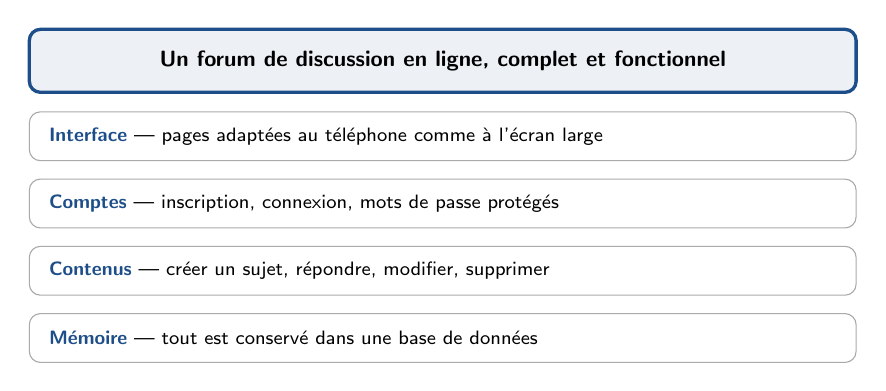
\begin{tikzpicture}[font=\scriptsize, node distance=0.22cm]
    \node[draw=accentBlue, very thick, rounded corners, fill=accentBlue!8,
          minimum width=10.5cm, minimum height=0.8cm, align=center] (a)
      {\footnotesize\textbf{Un forum de discussion en ligne, complet et fonctionnel}};
    \node[draw=cfptDarkGrey!50, rounded corners, fill=white,
          minimum width=10.5cm, minimum height=0.62cm, align=left,
          below=of a, text width=10cm] (b)
      {\textcolor{accentBlue}{\textbf{Interface}} --- pages adaptées au téléphone comme à l'écran large};
    \node[draw=cfptDarkGrey!50, rounded corners, fill=white,
          minimum width=10.5cm, minimum height=0.62cm, align=left,
          below=of b, text width=10cm] (c)
      {\textcolor{accentBlue}{\textbf{Comptes}} --- inscription, connexion, mots de passe protégés};
    \node[draw=cfptDarkGrey!50, rounded corners, fill=white,
          minimum width=10.5cm, minimum height=0.62cm, align=left,
          below=of c, text width=10cm] (d)
      {\textcolor{accentBlue}{\textbf{Contenus}} --- créer un sujet, répondre, modifier, supprimer};
    \node[draw=cfptDarkGrey!50, rounded corners, fill=white,
          minimum width=10.5cm, minimum height=0.62cm, align=left,
          below=of d, text width=10cm] (e)
      {\textcolor{accentBlue}{\textbf{Mémoire}} --- tout est conservé dans une base de données};
  \end{tikzpicture}
  \end{center}
  \vspace{-0.15cm}
  \begin{block}{Et vous saurez l'expliquer}
    \small La dernière séance est une soutenance : vous ferez fonctionner votre forum en direct et vous répondrez aux questions sur votre propre code.
  \end{block}
\end{frame}

\begin{frame}{Le chemin que parcourt une information}
  \begin{center}
  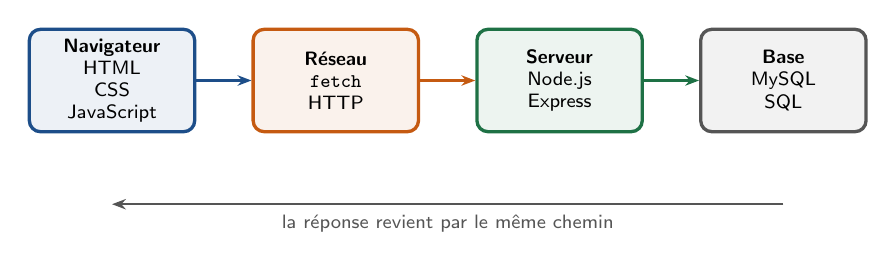
\begin{tikzpicture}[font=\scriptsize, node distance=0.7cm]
    \node[draw=accentBlue, very thick, rounded corners, fill=accentBlue!8,
          minimum width=2.1cm, minimum height=1.3cm, align=center] (nav)
      {\textbf{Navigateur}\\HTML\\CSS\\JavaScript};
    \node[draw=warningOrange, very thick, rounded corners, fill=warningOrange!8,
          minimum width=2.1cm, minimum height=1.3cm, align=center, right=of nav] (net)
      {\textbf{Réseau}\\\texttt{fetch}\\HTTP};
    \node[draw=successGreen, very thick, rounded corners, fill=successGreen!8,
          minimum width=2.1cm, minimum height=1.3cm, align=center, right=of net] (srv)
      {\textbf{Serveur}\\Node.js\\Express};
    \node[draw=cfptDarkGrey, very thick, rounded corners, fill=cfptGrey,
          minimum width=2.1cm, minimum height=1.3cm, align=center, right=of srv] (db)
      {\textbf{Base}\\MySQL\\SQL};
    \draw[-{Stealth[length=5pt]}, thick, accentBlue] (nav) -- (net);
    \draw[-{Stealth[length=5pt]}, thick, warningOrange] (net) -- (srv);
    \draw[-{Stealth[length=5pt]}, thick, successGreen] (srv) -- (db);
    \draw[-{Stealth[length=5pt]}, thick, cfptDarkGrey]
      ([yshift=-0.9cm]db.south)
      -- node[below, font=\scriptsize, text=cfptDarkGrey]
             {la réponse revient par le même chemin}
      ([yshift=-0.9cm]nav.south);
  \end{tikzpicture}
  \end{center}
  \vspace{0.3cm}
  \begin{block}{Ces quatre cases sont le plan du cours}
    On les apprend dans cet ordre, de gauche à droite. Chaque case est un morceau du même projet, pas un exercice isolé.
  \end{block}
\end{frame}

\begin{frame}{Ce que ce cours n'est pas}
  \begin{columns}[T]
    \begin{column}{0.48\textwidth}
      \begin{alertblock}{Pas un cours d'outils}
        Aucun framework à la mode. On écrit du HTML, du CSS et du JavaScript standard.
        \medskip

        La raison est simple : les outils changent tous les trois ans, les mécanismes en dessous, non.
      \end{alertblock}
    \end{column}
    \begin{column}{0.48\textwidth}
      \begin{block}{Un cours de raisonnement}
        Ce que vous emportez d'ici, c'est la capacité à découper un problème et à écrire la suite d'instructions qui le résout.
        \medskip

        C'est exactement ce qu'on vous demandera en première année à hepia.
      \end{block}
    \end{column}
  \end{columns}
\end{frame}

% ===============================================================
\sectionslide{2. Le parcours en 20 semaines}
% ===============================================================

\begin{frame}{Quatre phases, 20 semaines}
  \begin{center}
  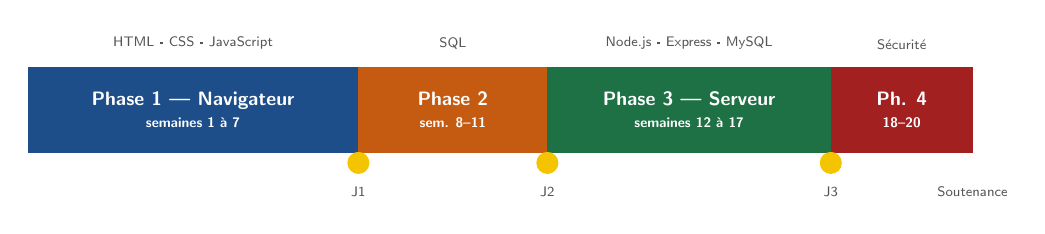
\begin{tikzpicture}[font=\scriptsize]
    % barres proportionnelles : 7 / 4 / 6 / 3 semaines sur 12 cm
    \fill[accentBlue]    (0,0)    rectangle (4.2,1.1);
    \fill[warningOrange] (4.2,0)  rectangle (6.6,1.1);
    \fill[successGreen]  (6.6,0)  rectangle (10.2,1.1);
    \fill[alertRed]      (10.2,0) rectangle (12,1.1);

    \node[text=white, font=\bfseries\scriptsize, align=center] at (2.1,0.55)
      {Phase 1 --- Navigateur\\{\tiny semaines 1 à 7}};
    \node[text=white, font=\bfseries\scriptsize, align=center] at (5.4,0.55)
      {Phase 2\\{\tiny sem. 8--11}};
    \node[text=white, font=\bfseries\scriptsize, align=center] at (8.4,0.55)
      {Phase 3 --- Serveur\\{\tiny semaines 12 à 17}};
    \node[text=white, font=\bfseries\scriptsize, align=center] at (11.1,0.55)
      {Ph. 4\\{\tiny 18--20}};

    % jalons
    \foreach \x/\l in {4.2/J1, 6.6/J2, 10.2/J3} {
      \fill[cfptYellow] (\x,-0.12) circle (0.14);
      \node[font=\tiny, text=cfptDarkGrey, below] at (\x,-0.3) {\l};
    }
    \node[font=\tiny, text=cfptDarkGrey, below] at (12,-0.3) {Soutenance};

    % légende contenu
    \node[align=center, font=\tiny, text=cfptDarkGrey, above] at (2.1,1.2) {HTML · CSS · JavaScript};
    \node[align=center, font=\tiny, text=cfptDarkGrey, above] at (5.4,1.2) {SQL};
    \node[align=center, font=\tiny, text=cfptDarkGrey, above] at (8.4,1.2) {Node.js · Express · MySQL};
    \node[align=center, font=\tiny, text=cfptDarkGrey, above] at (11.1,1.2) {Sécurité};
  \end{tikzpicture}
  \end{center}
  \vspace{0.5cm}
  \begin{columns}[T]
    \begin{column}{0.48\textwidth}
      \begin{block}{Rythme hebdomadaire}
        3 heures de théorie \quad + \quad 4 heures de pratique
      \end{block}
    \end{column}
    \begin{column}{0.48\textwidth}
      \begin{block}{Travail personnel}
        2 à 3 heures par semaine en dehors des cours
      \end{block}
    \end{column}
  \end{columns}
\end{frame}

\begin{frame}{Phase 1 --- Faire apparaître quelque chose à l'écran}
  \textbf{Semaines 1 à 7} \quad\textcolor{cfptDarkGrey}{\textbar}\quad 49 heures
  \medskip

  \begin{columns}[T]
    \begin{column}{0.55\textwidth}
      \begin{itemize}
        \item \textbf{S1} --- Comment marche le web, installation des outils, Git
        \item \textbf{S2--S3} --- HTML : structurer une page, les formulaires
        \item \textbf{S4--S5} --- CSS : mise en forme, adaptation au mobile
        \item \textbf{S6--S7} --- JavaScript : la logique, puis rendre la page vivante
      \end{itemize}
    \end{column}
    \begin{column}{0.42\textwidth}
      \begin{block}{Le retour est immédiat}
        Vous modifiez une ligne, vous rechargez, vous voyez le résultat. C'est ce qui rend cette phase agréable.
      \end{block}
    \end{column}
  \end{columns}
\end{frame}

\begin{frame}{Fin de la semaine 7 --- le moment charnière}
  \begin{center}
  
\begin{tikzpicture}[font=\small]
    \node[draw=accentBlue, very thick, rounded corners, fill=accentBlue!8,
          text width=5cm, align=center, minimum height=1.8cm] (a)
      {Votre forum fonctionne.\\Vous ajoutez un sujet,\\il apparaît à l'écran.};
    \node[draw=alertRed, very thick, rounded corners, fill=alertRed!8,
          text width=5cm, align=center, minimum height=1.8cm, right=1.4cm of a] (b)
      {Vous rechargez la page.\\\textbf{Tout a disparu.}};
    \draw[-{Stealth[length=7pt]}, very thick, cfptDarkGrey] (a) -- (b);
  \end{tikzpicture}
  \end{center}
  \vspace{0.4cm}
  \begin{alertblock}{C'est voulu}
    Ce n'est pas un bug, et ce n'est pas votre faute. Un navigateur ne retient rien. Pour qu'une information survive, il faut la ranger ailleurs --- dans une base de données. C'est exactement là que commence la phase 2.
  \end{alertblock}
\end{frame}

\begin{frame}{Phase 2 --- Donner une mémoire au forum}
  \textbf{Semaines 8 à 11} \quad\textcolor{cfptDarkGrey}{\textbar}\quad 28 heures
  \medskip

  \begin{columns}[T]
    \begin{column}{0.55\textwidth}
      \begin{itemize}
        \item \textbf{S8} --- Dessiner la structure des données avant de coder
        \item \textbf{S9--S10} --- Interroger : retrouver, trier, compter, croiser
        \item \textbf{S11} --- Modifier : ajouter, mettre à jour, supprimer
      \end{itemize}
      \medskip
      C'est la partie la plus abstraite du cours. Elle reçoit quatre semaines pour cette raison.
    \end{column}
    \begin{column}{0.42\textwidth}
      \begin{block}{Une compétence qui dépasse le web}
        Les bases de données sont derrière à peu près tout : une banque, un site de billets, un dossier médical.
      \end{block}
    \end{column}
  \end{columns}
\end{frame}

\begin{frame}{Phase 3 --- Relier les deux}
  \textbf{Semaines 12 à 17} \quad\textcolor{cfptDarkGrey}{\textbar}\quad 42 heures
  \medskip

  \begin{columns}[T]
    \begin{column}{0.55\textwidth}
      \begin{itemize}
        \item \textbf{S12} --- Attendre une réponse qui met du temps à venir
        \item \textbf{S13} --- Construire votre propre serveur
        \item \textbf{S14--S15} --- Le brancher sur la base de données
        \item \textbf{S16} --- Le brancher sur votre interface
        \item \textbf{S17} --- Ranger, relire, réparer
      \end{itemize}
    \end{column}
    \begin{column}{0.42\textwidth}
      \begin{block}{La phase la plus dense}
        C'est ici que les trois morceaux se rejoignent. À la fin de la semaine 16, votre forum fonctionne vraiment.
      \end{block}
    \end{column}
  \end{columns}
\end{frame}

\begin{frame}{Phase 4 --- Le rendre sérieux}
  \textbf{Semaines 18 à 20} \quad\textcolor{cfptDarkGrey}{\textbar}\quad 21 heures
  \medskip

  \begin{columns}[T]
    \begin{column}{0.55\textwidth}
      \begin{itemize}
        \item \textbf{S18} --- Comptes, connexion, mots de passe protégés
        \item \textbf{S19} --- Se défendre contre les attaques les plus courantes
        \item \textbf{S20} --- Finalisation et soutenances
      \end{itemize}
    \end{column}
    \begin{column}{0.42\textwidth}
      \begin{alertblock}{Un mot de passe ne se stocke jamais tel quel}
        On verra pourquoi, et ce qui arrive aux entreprises qui l'ont oublié.
      \end{alertblock}
    \end{column}
  \end{columns}
\end{frame}

% ===============================================================
\sectionslide{3. Le projet fil rouge}
% ===============================================================

\begin{frame}{Un seul projet, du premier au dernier jour}
  \begin{columns}[T]
    \begin{column}{0.48\textwidth}
      \begin{alertblock}{Ce qu'on ne fera pas}
        Une série d'exercices sans lien, oubliés une semaine après avoir été rendus.
      \end{alertblock}
    \end{column}
    \begin{column}{0.48\textwidth}
      \begin{block}{Ce qu'on fera}
        \textbf{MiniForum} : un forum que vous commencez en semaine 1 et que vous présentez en semaine 20.
      \end{block}
    \end{column}
  \end{columns}
  \vspace{0.4cm}
  \begin{center}
  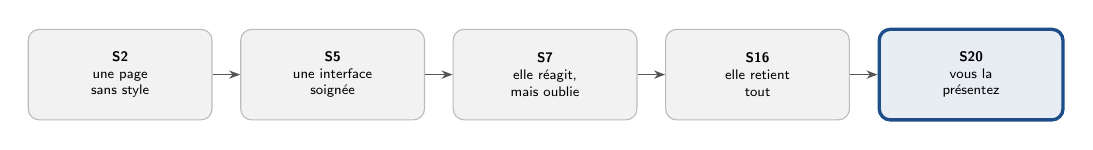
\begin{tikzpicture}[font=\tiny, node distance=0.35cm]
    \node[draw=cfptDarkGrey!40, rounded corners, fill=cfptGrey, text width=2.1cm,
          align=center, minimum height=1.15cm] (n1) {\textbf{S2}\\une page\\sans style};
    \node[draw=cfptDarkGrey!40, rounded corners, fill=cfptGrey, text width=2.1cm,
          align=center, minimum height=1.15cm, right=of n1] (n2) {\textbf{S5}\\une interface\\soignée};
    \node[draw=cfptDarkGrey!40, rounded corners, fill=cfptGrey, text width=2.1cm,
          align=center, minimum height=1.15cm, right=of n2] (n3) {\textbf{S7}\\elle réagit,\\mais oublie};
    \node[draw=cfptDarkGrey!40, rounded corners, fill=cfptGrey, text width=2.1cm,
          align=center, minimum height=1.15cm, right=of n3] (n4) {\textbf{S16}\\elle retient\\tout};
    \node[draw=accentBlue, very thick, rounded corners, fill=accentBlue!10, text width=2.1cm,
          align=center, minimum height=1.15cm, right=of n4] (n5) {\textbf{S20}\\vous la\\présentez};
    \foreach \a/\b in {n1/n2, n2/n3, n3/n4, n4/n5}
      \draw[-{Stealth[length=4pt]}, cfptDarkGrey] (\a) -- (\b);
  \end{tikzpicture}
  \end{center}
  \vspace{0.2cm}
  \centerline{\small Rien n'est jeté. Ce que vous écrivez en semaine 6 sert encore en semaine 20.}
\end{frame}

\begin{frame}{Si vous décrochez, vous pouvez remonter dans le train}
  \begin{block}{Le risque d'un projet filé sur 20 semaines}
    Vous bloquez en semaine 4, et vous ne rattrapez plus jamais. C'est le danger de ce format, et je le prends au sérieux.
  \end{block}
  \vspace{0.3cm}
  \begin{center}
  
\begin{tikzpicture}[font=\scriptsize, node distance=1.2cm]
    \node[draw=successGreen, very thick, rounded corners, fill=successGreen!8,
          minimum width=2.6cm, minimum height=1cm, align=center] (d1) {\textbf{Semaine 7}\\dépôt fourni};
    \node[draw=successGreen, very thick, rounded corners, fill=successGreen!8,
          minimum width=2.6cm, minimum height=1cm, align=center, right=of d1] (d2) {\textbf{Semaine 11}\\dépôt fourni};
    \node[draw=successGreen, very thick, rounded corners, fill=successGreen!8,
          minimum width=2.6cm, minimum height=1cm, align=center, right=of d2] (d3) {\textbf{Semaine 17}\\dépôt fourni};
  \end{tikzpicture}
  \end{center}
  \vspace{0.3cm}
  \begin{exampleblock}{Comment ça marche}
    À la fin de chaque phase, je publie un MiniForum conforme à ce qui était attendu. Si votre projet est en difficulté, vous repartez du mien pour la phase suivante --- sans pénalité sur la suite.
    \medskip

    Prendre du retard est normal. Rester bloqué dehors ne l'est pas.
  \end{exampleblock}
\end{frame}

% ===============================================================
\sectionslide{4. L'évaluation}
% ===============================================================

\begin{frame}{Comment la note se construit}
  \begin{center}
  \renewcommand{\arraystretch}{1.25}
  \begin{tabularx}{0.92\textwidth}{lXcc}
    \toprule
    \rowcolor{accentBlue}
    \color{white}\textbf{Épreuve} & \color{white}\textbf{Ce qui est évalué} &
    \color{white}\textbf{Sem.} & \color{white}\textbf{Poids} \\
    \midrule
    \rowcolor{cfptGrey}
    Jalon 1 & L'interface fonctionne dans le navigateur & 7 & 10\,\% \\
    Jalon 2 & Le modèle de données et les requêtes & 11 & 10\,\% \\
    \rowcolor{cfptGrey}
    Contrôle écrit & Individuel, sur machine, sans réseau & 12 & 25\,\% \\
    Jalon 3 & Le serveur est branché sur la base & 17 & 10\,\% \\
    \rowcolor{cfptGrey}
    Projet final & Le MiniForum complet & 20 & 30\,\% \\
    Soutenance & Vous le présentez et l'expliquez & 20 & 15\,\% \\
    \bottomrule
  \end{tabularx}
  \end{center}
  \vspace{0.05cm}
  \begin{block}{Les jalons sont là pour vous, pas contre vous}
    \small Ils pèsent peu volontairement. Leur rôle est de repérer tôt ce qui coince, pendant qu'il est encore temps d'y remédier.
  \end{block}
\end{frame}

\begin{frame}{La soutenance --- semaine 20}
  \begin{columns}[T]
    \begin{column}{0.46\textwidth}
      \textbf{10 minutes} de présentation\\
      \textbf{5 minutes} de questions
      \medskip

      \begin{itemize}
        \item Votre forum tourne en direct
        \item Vous expliquez ce que fait votre code
        \item Vous répondez aux questions
        \item Vous dites ce qui a été difficile
      \end{itemize}
    \end{column}
    \begin{column}{0.5\textwidth}
      \begin{block}{Ce qui compte}
        \begin{tabular}{@{}p{4.4cm}r@{}}
          Démonstration & 30\,\%\\
          Explication de votre code & 30\,\%\\
          Réponses aux questions & 25\,\%\\
          Clarté de la présentation & 15\,\%\\
        \end{tabular}
      \end{block}
      \medskip
      \centerline{\small Un projet qui marche mais}
      \centerline{\small que vous ne savez pas expliquer}
      \centerline{\small ne vaut que la moitié des points.}
    \end{column}
  \end{columns}
\end{frame}

% ===============================================================
\sectionslide{5. Les règles du jeu}
% ===============================================================

\begin{frame}{L'intelligence artificielle générative est interdite}
  \begin{alertblock}{La règle}
    Copilot, ChatGPT, Claude, Gemini et les autres assistants qui écrivent du code sont \textbf{interdits} pour tous les travaux de ce cours : TP, jalons, projet, contrôle écrit.
  \end{alertblock}
  \vspace{0.4cm}
  \begin{columns}[T]
    \begin{column}{0.48\textwidth}
      \begin{block}{Ce qui reste autorisé}
        \begin{itemize}
          \item La documentation officielle (MDN)
          \item Les moteurs de recherche, les forums
          \item Vous entraider --- chacun écrit son code
          \item Prettier, ESLint (mise en forme)
        \end{itemize}
      \end{block}
    \end{column}
    \begin{column}{0.48\textwidth}
      \begin{block}{Comment je le vérifie}
        \begin{itemize}
          \item Extensions désinstallées aujourd'hui
          \item Historique Git examiné aux jalons
          \item Questions orales sur votre code
          \item Contrôle écrit sans réseau
        \end{itemize}
      \end{block}
    \end{column}
  \end{columns}
\end{frame}

\begin{frame}{Pourquoi cette règle}
  \begin{columns}[T]
    \begin{column}{0.5\textwidth}
      \begin{block}{Là où l'apprentissage se produit}
        On apprend à programmer en écrivant du code, en le voyant échouer, et en comprenant pourquoi.
        \medskip

        Un assistant qui donne la bonne réponse tout de suite supprime précisément cette étape.
      \end{block}
    \end{column}
    \begin{column}{0.46\textwidth}
      \begin{alertblock}{L'enjeu est concret}
        En première année à hepia, les épreuves de programmation sont individuelles et sans assistance.
        \medskip

        Arriver avec un beau projet et aucune des compétences correspondantes, c'est arriver désarmé.
      \end{alertblock}
    \end{column}
  \end{columns}
  \vspace{0.35cm}
  \begin{exampleblock}{Ce n'est pas un refus de l'outil}
    Ces assistants font partie du métier, et vous les utiliserez. Mais on ne les utilise utilement qu'une fois qu'on sait lire ce qu'ils produisent. On en reparle en semaine 20.
  \end{exampleblock}
\end{frame}

\begin{frame}{Git --- votre trace de travail}
  \begin{columns}[T]
    \begin{column}{0.52\textwidth}
      \begin{itemize}
        \item Vous créez votre dépôt aujourd'hui
        \item Vous y déposez votre travail \textbf{à chaque séance}
        \item L'historique est regardé aux jalons
        \item Il compte dans la note du projet final
      \end{itemize}
      \medskip
      Ce n'est pas une formalité administrative : c'est ce qui vous permettra de revenir en arrière quand vous casserez quelque chose. Et vous casserez quelque chose.
    \end{column}
    \begin{column}{0.44\textwidth}
      \begin{alertblock}{Un projet livré en un seul dépôt massif}
        \dots donne lieu à un entretien.
      \end{alertblock}
    \end{column}
  \end{columns}
\end{frame}

% ===============================================================
\sectionslide{6. Et après ? hepia}
% ===============================================================

\begin{frame}{Ce que ce cours prépare vraiment}
  \begin{alertblock}{Soyons clairs}
    Le développement web n'est pas enseigné en première année à hepia. Il arrive au semestre 4, en orientation informatique logicielle.
  \end{alertblock}
  \vspace{0.3cm}
  \begin{block}{Alors pourquoi ce cours ?}
    Parce que le web est le moyen le plus rapide de vous faire écrire beaucoup de code en voyant tout de suite le résultat. Ce que vous emportez, ce n'est pas le HTML : c'est l'habitude de raisonner comme un programmeur.
  \end{block}
  \vspace{0.3cm}
  \begin{center}
  \small
  \begin{tabular}{@{}ll@{}}
    \textcolor{accentBlue}{\textbf{Algorithmique et programmation}} & votre matière la plus lourde en 1\textsuperscript{re} année\\
    \textcolor{accentBlue}{\textbf{Réseaux et sécurité}} & client/serveur, HTTP, mots de passe\\
    \textcolor{accentBlue}{\textbf{Systèmes de bases de données}} & semestre 4\\
    \textcolor{accentBlue}{\textbf{Développement web}} & semestre 4, orientation logicielle\\
  \end{tabular}
  \end{center}
\end{frame}

\begin{frame}{Concrètement, à partir de maintenant}
  \begin{columns}[T]
    \begin{column}{0.48\textwidth}
      \begin{block}{Aujourd'hui}
        \begin{itemize}
          \item Comment fonctionne le web
          \item Installation de vos outils
          \item Création de votre dépôt Git
          \item Premier commit de MiniForum
        \end{itemize}
      \end{block}
    \end{column}
    \begin{column}{0.48\textwidth}
      \begin{block}{À votre disposition}
        \begin{itemize}
          \item Le plan de cours complet (PDF)
          \item Un polycopié par semaine
          \item Les corrigés des exercices
          \item Les dépôts de référence
        \end{itemize}
      \end{block}
    \end{column}
  \end{columns}
  \vspace{0.4cm}
  \begin{exampleblock}{Une chose à retenir de cette présentation}
    Personne ici ne part avec de l'avance. Ce qui fera la différence en juin, c'est le nombre d'heures que vous aurez passées les mains dans le code --- pas le talent.
  \end{exampleblock}
\end{frame}

{
\setbeamertemplate{footline}{}
\begin{frame}[plain]
  \begin{tikzpicture}[remember picture, overlay]
    \fill[accentBlue] (current page.north west) rectangle (current page.south east);
    \node[text=white, font=\Huge\bfseries] at ([yshift=0.6cm]current page.center) {Des questions ?};
    \fill[cfptYellow] ([yshift=-0.2cm]current page.center -| current page.west)
      rectangle ([yshift=-0.32cm]current page.center -| current page.east);
    \node[text=lightBlue, font=\large] at ([yshift=-1.3cm]current page.center)
      {On enchaîne : semaine 1 --- fondamentaux du web};
  \end{tikzpicture}
\end{frame}
}

\end{document}
